\section{Bau zwei verschiedener Fernrohre}
\subsection{Keplersches Fernrohr}

In diesem Versuchsteil geht es darum ein Keplersches Fernrohr zu bauen und dabei mindestens eine Vergrößerung von 6 zu erreichen. Dazu werden zwei Linsen mit verschiedenen Brennweiten so auf einer optische Bank befestigt, dass sie einen Abstand von $$ d = f_1 + f_2 $$ haben. Um die gewünschte Vergrößerung zu erreichen wählt man die Linsen so, dass die Formel für die Vergrößerung mindestens 6 ergibt. $$  \gamma = \frac{f_1}{f_2} \geqslant 6$$. Gewählt wird eine für die erste Linse eine Brennweite von $500mm$ und für die zweite eine Brennweite von $70mm$, was eingesetzt in die Formel für die Vergrößerung eine theoretische Vergrößerung von $\thickapprox 7,14 $ ergibt. Der Abstand zwischen den Linsen muss demnach $d = 700mm + 50mm = 57cm$ betragen.
Um die experimentelle Vergrößerung zu ermitteln wird der Okulardurchmesser gemessen und der durch das Fernrohr sichtbare Bereich gemessen, dies entspricht der Bild- und Gegenstandsgröße, somit kann mit der Formel $$ \gamma = \frac{B}{G} $$ die Vergrößerung berechnet werden. Mit den Werten aus der Tabelle \ref{tab:Tabellekeppler} ergibt sich eine Vergrößerung von $10$. Was einer relativ großen Abweichung vom theoretischen Wert entspricht. Was wahrscheinlich auf die ungenaue Methode die Vergrößerung zu messen zurückzuführen ist.

\begin{table}[h]
    \centering
    \begin{tabular}{|c|c|}
	\hline
	f1\ & 500mm \\
	\hline
	f2\ & 70mm \\
	\hline
	Theoretische Vergrößerung  & 7,14 \\
	\hline
	Okulardurchmesser & 31mm \\
	\hline
	Sichtbarer Bereich & 310mm \\
	\hline
	Exp. gemessene Vergrößerung & 10 \\
	\hline
    \end{tabular}
    \caption{Messwerte Keplersches Fernrohr}
    \label{tab:Tabellekeppler}
\end{table}

\begin{figure}
    \centering
    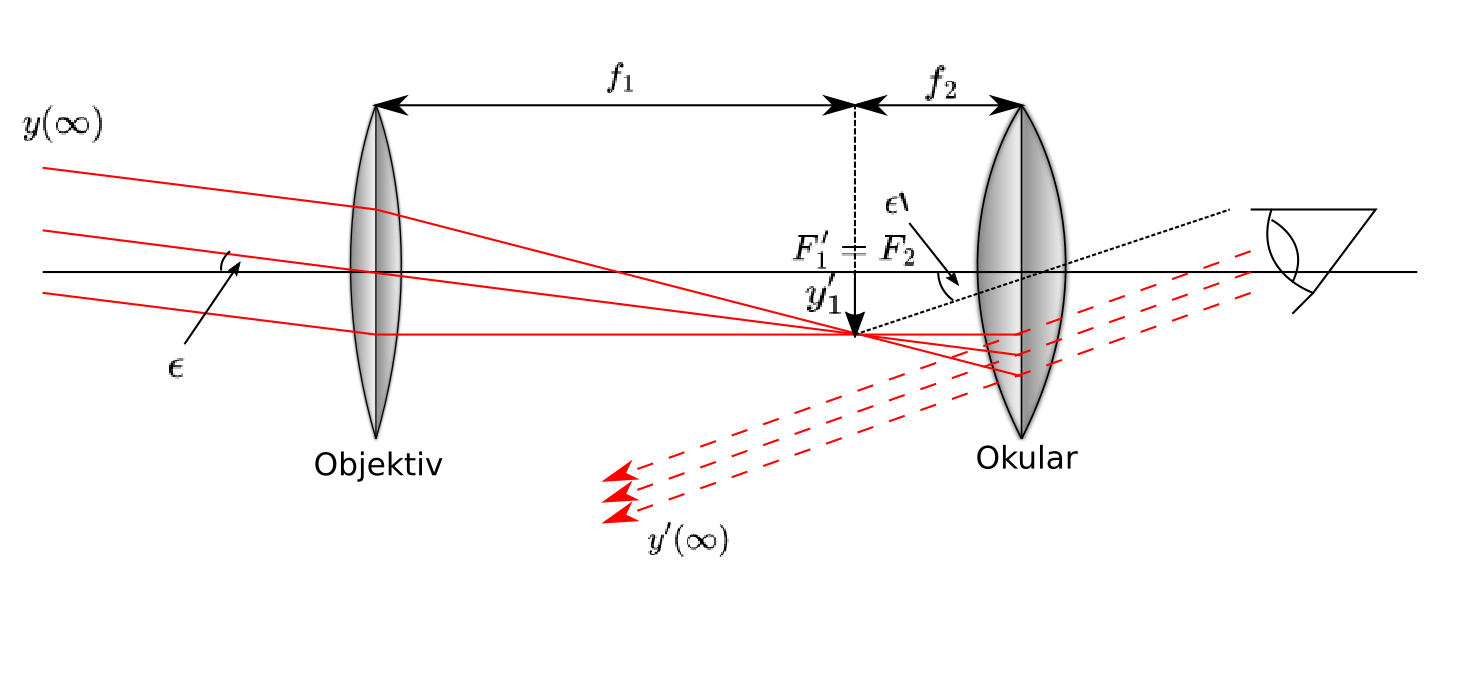
\includegraphics[scale=0.8]{Geometrische_Optik/Protokoll/fig/Keplerfernrohr.png}
    \caption{Keplerfernrohr}
    \label{fig:Keplerfernrohr}
\end{figure}

\subsection{Galileisches Fernrohr}
Die Besonderheit des Galileischen Fernrohrs gegenüber dem Keplerschen, ist, dass es sich eine Zerstreuungslinse zur Nutze macht, dadurch steht das Bild nicht mehr auf dem Kopf, außerdem lässt sich mit dieser Bauart eine geringe Baulänge erreichen bei gleicher Vergrößerung. Die Vergrößerung lässt sich ähnlich wie beim Galileischen Fernrohr berechnen: $$ \gamma = \frac{f_1}{|f_2|} $$ Wobei die Baulänge und somit der Abstand der Linsen $$ d = f_1' - |f_2| $$ beträgt. Für diesen Versuch werden Linsen mit den Brennweiten $f_1 = 500$ und $f_2 = -100$ gewählt. Nach obiger Formel müssen die Linsen einen Abstand von $400mm$ haben. Errechnet werden wieder theoretische Vergrößerung und experimentell bestimmte Vergrößerung, es ergeben sich die in Tabelle \ref{tab:Tabellegalileo} aufgeführten Werte.

\begin{table}[h]
    \centering
\begin{tabular}{|c|c|}
	\hline
	f1 & 500mm \\
	\hline
	f2 & -10mm \\
	\hline
	Theoretische Vergrößerung & 5 \\
	\hline
	Okulardurchmesser & 8mm \\
	\hline
	Sichtbarer Bereich & 341mm \\
	\hline
	Exp. gemessene Vergrößerung & 4.26 \\
	\hline
    \end{tabular}
    \caption{Messwerte Gelileisches Fernrohr}
    \label{tab:Tabellegalileo}
\end{table}

\begin{figure}
    \centering
    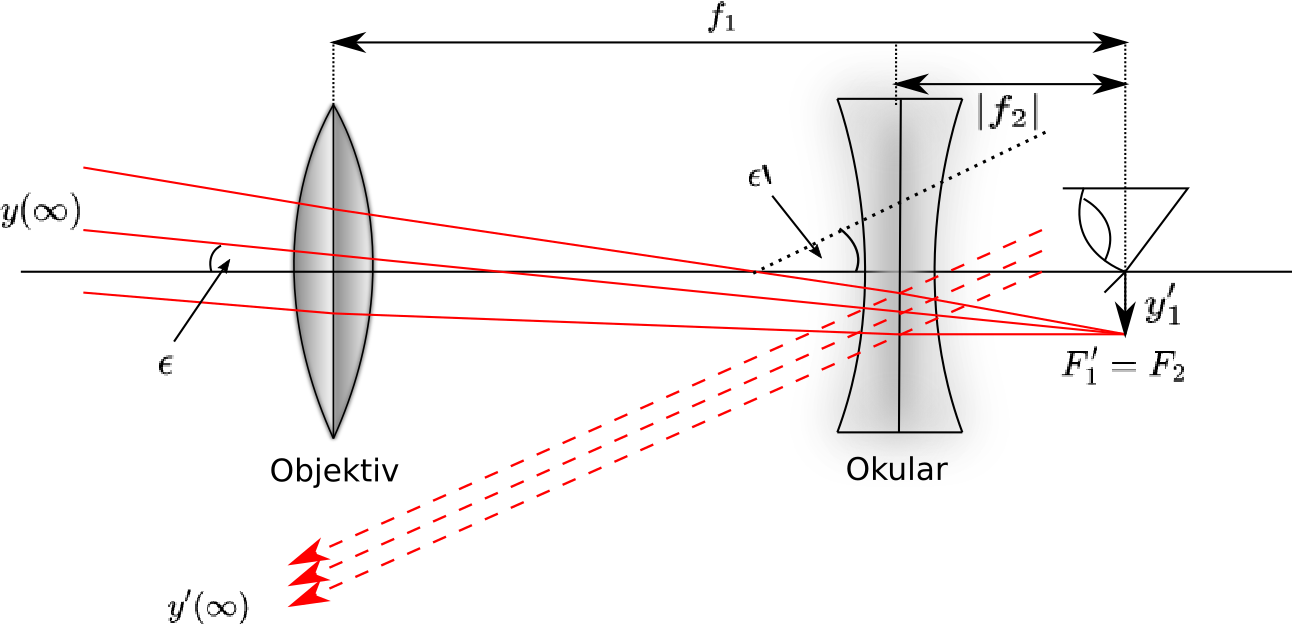
\includegraphics[scale=0.8]{Geometrische_Optik/Protokoll/fig/Galileofernrohr.png}
    \caption{Galileofernrohr}
    \label{fig:Galileofernrohr}
\end{figure}

\section{Bau eines Projektionsapparats}

\begin{figure}
    \centering
    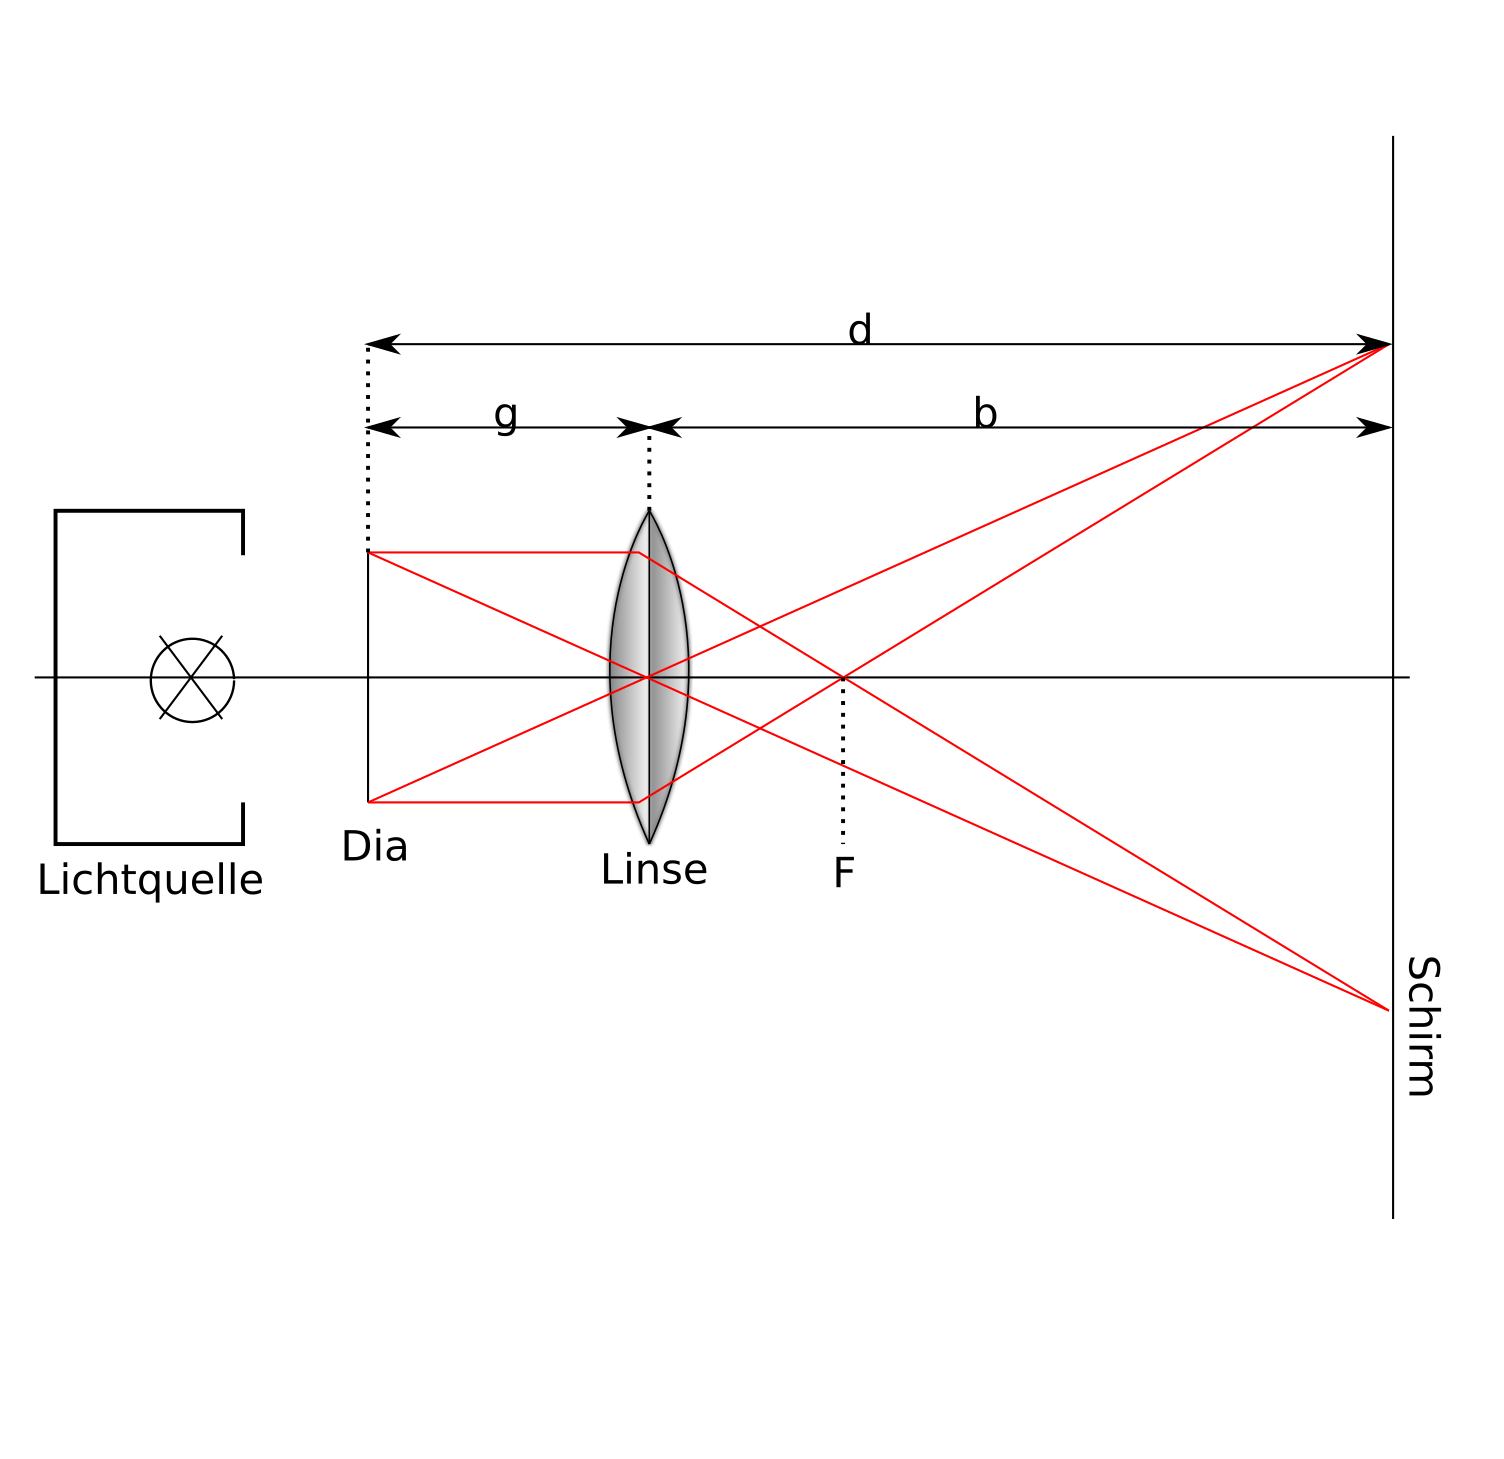
\includegraphics[scale=0.8]{Geometrische_Optik/Protokoll/fig/Diaprojektor.png}
    \caption{Diaprojektor}
    \label{fig:Diaprojektor}
\end{figure}

\section{Bau eines Mikroskops}

\begin{figure}
    \centering
    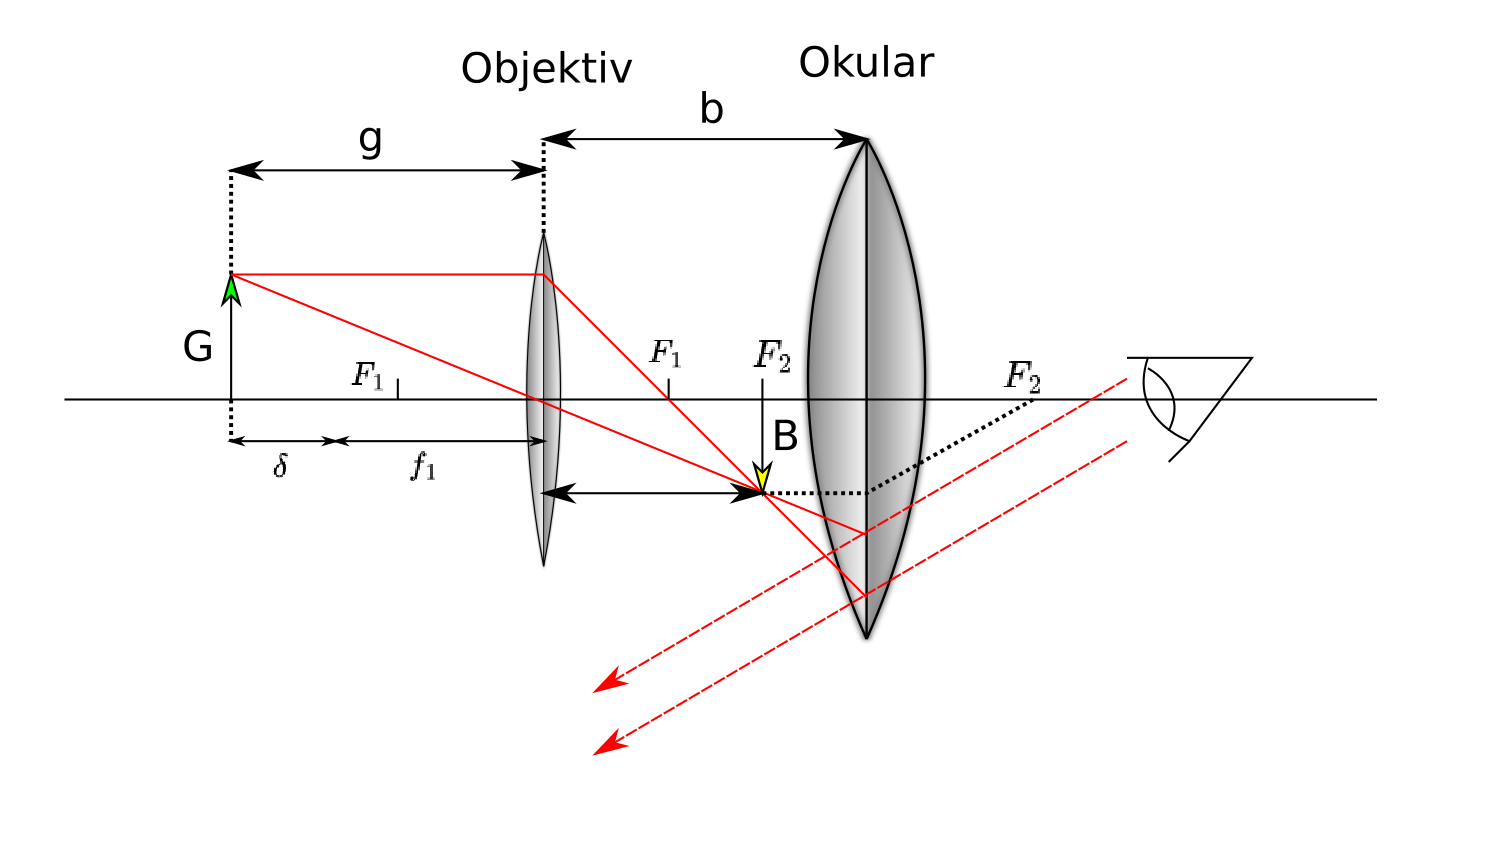
\includegraphics[scale=0.8]{Geometrische_Optik/Protokoll/fig/Mikroskop.png}
    \caption{Mikroskop}
    \label{fig:Mikroskop}
\end{figure}